\documentclass[12pt]{article}
\usepackage{amsmath, amsthm, latexsym, tikz, graphicx, listings, microtype, mathtools, soul, color, fancyhdr}
\usepackage[margin=1in]{geometry}
\usepackage[utf8]{inputenc}

\newenvironment{myindentpar}[1]%
 {\begin{list}{}%
         {\setlength{\leftmargin}{#1}}%
         \item[]%
 }
 {\end{list}}

\DeclarePairedDelimiter\abs{\lvert}{\rvert}%
\DeclarePairedDelimiter\norm{\lVert}{\rVert}%

% Swap the definition of \abs* and \norm*, so that \abs
% and \norm resizes the size of the brackets, and the
% starred version does not.
\makeatletter
\let\oldabs\abs
\def\abs{\@ifstar{\oldabs}{\oldabs*}}
%
\let\oldnorm\norm
\def\norm{\@ifstar{\oldnorm}{\oldnorm*}}
\makeatother

\definecolor{lightgray}{gray}{0.65}
\definecolor{pinegreen}{RGB}{1, 171, 161}
\definecolor{lightblue}{RGB}{135, 206, 250}
\definecolor{dkgreen}{rgb}{0,0.6,0}
\definecolor{gray}{rgb}{0.5,0.5,0.5}
\definecolor{mauve}{rgb}{0.58,0,0.82}
\definecolor{darkblue}{rgb}{0.0,0.0,0.6}
\definecolor{cyan}{rgb}{0.0,0.6,0.6}

\newcommand*{\Value}{\frac{1}{2}x^2}%
\newcommand{\hlc}[2][yellow]{ {\sethlcolor{#1} \hl{#2}} }


% /*--------------------------------------------------------------*/
%   Changing the values here sets the due date for the assignment!
% /*--------------------------------------------------------------*/
\newcommand{\duedate}{4/8/21 Thursday at 11:59pm}
\newcommand{\semester}{Spring 2021}

\lstset{frame=tb,
  language=C++,
  breaklines=true,
  showstringspaces=false,
  columns=flexible,
  numbers=none,
  tabsize=3,
  escapeinside={(*@}{@*)}
  %,
  %commentstyle=\color{dkgreen},
  %stringstyle=\color{mauve}
}
\lstdefinestyle{bash}
{ language=bash,
  aboveskip=3mm,
  belowskip=3mm,
  showstringspaces=false,
  columns=flexible,
  basicstyle={\small\ttfamily\color{green}}, 
  numbers=none,
  numberstyle=\tiny\color{gray},
  keywordstyle=\color{blue},
  commentstyle=\color{dkgreen},
  stringstyle=\color{mauve},
  breaklines=true,
  breakatwhitespace=true,
  tabsize=3,
  backgroundcolor=\color{black},
}

% \usepackage[most]{tcolorbox}
% \newtcblisting{commandshell}{colback=black,colupper=white,colframe=yellow!75!black,
% listing only,listing options={language=sh, style=tcblatex},
% every listing line={\textcolor{green}{\small\ttfamily\bfseries prompt \$> }}}
\pagestyle{fancy}
\fancyhf{}

\renewcommand{\headrulewidth}{0pt}
\lhead{\color{lightgray} CSCE 313}
\rhead{\color{lightgray} \semester}
\rfoot{\thepage}
\pagenumbering{arabic}

\definecolor{codegray}{gray}{0.9}
\newcommand{\code}[1]{\colorbox{codegray}{\texttt{#1}}}

\begin{document}
\title{PA\#4: Threading and Synchronization}
\date{\vspace{-5ex}Due: \duedate}
\maketitle

\section*{Introduction}
In this programming assignment, you would increase the efficiency of your PA1. You may have noticed that PA1 takes a long time to collect $1$K data requests per person. It would take much longer to collect all requests in a single file. Transferring raw files through file messages, although faster than using data messages, is still quite slow because of single channel usage at a time. In PA3, we learned how to create multiple channels, which the server processes independently and in parallel. However, we could not take advantage of that because our client program in PA3 was single-threaded. In this PA, you would incorporate multiple threads to make these operations significantly faster. 

\section*{Threading for Faster Programs}
The primary bottleneck in PA1 for collecting data points is the fact that we must collect data points one after another. This problem is worsened further by the random processing time of each request (i.e., emulated using a \texttt{usleep()} call) by the server. And since the requests are all sequential, one delayed request-response would affect all subsequent requests. Notice in the \texttt{BIMDC/} directory that there are $15$ files, one for each patient. One way to collect data faster from these files is  to use $15$ threads from the client side, one for each patient. Each thread would create its own request channel with the server and then independently collect the responses for a person. Since the server already processes each channel in a separate thread, you can get atmost $15$-fold speed over the sequential version. This technique is shown in Figure \ref{fig:first}. Note that file requests can be spedup similarly.  


\begin{figure}[t]\centering
	\includegraphics[width=5in]{first.eps}
	\caption{First approach to scaling PA1 performance - one thread per patient.}
	\label{fig:first}
  \end{figure}

However, there is a big problem: even if there are adequate hardware resources (e.g., CPU cores), you cannot use more than $p$-fold speedup, where $p$ is the number of patients you are collecting data for. In addition, since each request takes a random time, some patient threads may take much longer compared to the other ones. To avoid this roadblock, we have to make the number of threads some how indpendent of the number of patients $p$. 

The standard solution to this problem is to separate the tasks of \emph{producing} these requests and \emph{processing} them (i.e., sending to the server), and using a buffer in between these tasks. This way the number of patients $p$ can be decoupled from the number of threads that would be in charge of communicating with the server, simplifying the scaling issue. That means now there are $p$ \texttt{patient} threads pushing requests on to the buffer, which can be thought of an \texttt{STL::queue}. Then, there are $w$ \texttt{worker} threads, each communicating with the server independently of each other through a dedicated request channel. As a result, the theoretical speedup factor is now $w$, which is indpendent of $p$ and can lead to significantly more speedup with $w >> p$. Figure \ref{fig:second} demonstrates this technique.

\begin{figure}[t]\centering
	\includegraphics[width=5in]{second.eps}
	\caption{Second try with a buffer - number of worker threads $w$ is now independent of number of patients $p$.}
	\label{fig:second}
  \end{figure}

For this technique to work, you need a special and more compilcated buffer than just an \texttt{STL queue} between the patient threads and the worker threads. First, the queue must be thread-safe; otherwise simultaneous accesses from the producers (i.e., patient threads) and consumers (i.e., worker threads) would lead to a race condition. Second, the buffer must be made ``bounded'' so that the memory footprint of the buffer is under check and does not grow to infinity. In summary, the buffer must be protected against ``race-conditions'', ``overflow'' and ``underflow''. Overflow can happen when the patient threads are much faster than the worker threads, while underflow can happen under the opposite scenario. As described in the ``Synchrnonization'' lecture, the \texttt{BoundedBuffer} class is the perfect solution to all these problems. 

\subsection*{Client Requesting Data Points}
The workers threads in this PA work as follows. Each worker thread pops a request from the request buffer (i.e., the \texttt{BoundedBuffer} object between the patient and the worker threads), sends it to the server, collects the response, and then puts the response in the response buffer - another \texttt{BoundedBuffer} object. In addition, there are $h$ histogram threads who pop these responses and update $p$ ecg histograms, one for each patient. 


There is a histogram per patient that keeps track of that patient's statistics. Note that multiple worker threads would potentially update the same histogram leading to another race condition, which must be avoided by using mutual exclusion.

In order for the histogram threads to know which response is for which patient, the worker threads make sure to prepend each data response with the respective patient no. You can do that by making a pair out of the patient no and the data response (i.e., using \texttt{STL::pair} or a separate struct/class with 2 fields). 


 Figure \ref{fig:PA3} shows the structure.

When requesting data messages, the program should take $4$ command line arguments: $n$ for number of data items (in range $[1,15K]$), $p$ for number of patients (range $[1,15]$), $w$ for number of worker threads (try between $[50, 5000]$), and $b$ for bounded buffer size in bytes (acceptable range $[100, 1000000]$). For instance, the following command is requesting $15$K ecg data for the first $10$ patients using $500$ worker threads and a request buffer of size 1KB (i.e., $1024$ bytes). It will use a 1KB response buffers to collect the responses and then $h=5$ histogram threads to make the $10$ patient histograms for ecg values.

%\begin{commandshell}
\begin{lstlisting}[style=bash]
	$./client -n 15000 -p 10 -h 5 -w 500 -b 1024
\end{lstlisting}

Note that all these arguments are optional, meaning that they can be omitted, causing their default values being used.

Notice that there is a total of $p+w+h$ threads in just the client program: $p$ patient threads, $w$ worker threads and $h$ histogram threads. All these threads must be running simultaneously for your program to work; otherwise the request and/or the response buffers will stall after reaching their bounds or after running dry. 

You cannot just use a huge request buffer where all requests would fit. Make sure to test your program using small request/response buffer size (e.g., $b=100$) - your program should work perfectly fine, may be a bit slower. Smaller $b$ values along with high $p, w, n, h$ increase concurrency and thus manifest race condition bugs that are not visible under easier circumstances. Make sure to stress-test your program under these settings.

\subsection*{Client Requesting Files}
You can also run the client for file requests. First, the client queries the file size just like PA1. After that, instead of sending the requests directly to the server, the client starts a thread that makes and puts all the requests on to the request buffer. The worker threads pop those requests from the buffer, send those out to the server through their dedicated request channels, receive the responses, and write those responses into the appropriate locations of the file. Note that unlike requesting data messages, there is no response buffer in this case. The structure is shown in Figure \ref{fig:PA3_file}. Note that while the progrm is running, there are $w+1$ threads working simultaneously: 1 thread for making the requests and pushing them to the request buffer, the rest $w$ worker threads who keep taking from the request buffer and process them.

Note that in this design, file chunks can be received out-of-order (earlier chunks arriving later or vice versa). You must make your worker threads robust such that they do not corrupt the file when they are writing to it simultaneously. There is a specific mode for opening a file that would make this possible.

When requesting a flie, the client would take 4 command line arguments: $w$ for the number of worker threads, $b$ for request buffer size, $m$ for buffer capacity to keep the file content in memory, and $f$ for file name. The first two are optional and the last argument (i.e, ``-f'') is mandatory. The following example command asks to download the file ``file.bin'' using $100$ worker threads and using a buffer capacity of $256$ bytes. 

\begin{lstlisting}[style=bash]
	./client -w 100 -f test.bin -m 256 -b 100
\end{lstlisting}	

Capacity $m$ indicates the maximum number of bytes from the file that can be sent back from the server in each response. Note that the \texttt{server} needs to know how this value, which would be passed from the \texttt{client} as a command line argument through the \texttt{exec()} function.  

You should vary $m$ and $w$ and report the variation in runtime that you experience for files of different sizes. Make sure to test your program using boundary conditions (e.g., $m=30, w=1$, or $m=30, w=5000$). You need the buffer capacity $m$ at least big enough for the name of a new channel or any other messages exchanged between the client and the server. 


\subsection*{Implementing the BoundedBuffer}
\texttt{BoundedBuffer} must use an STL queue of items to maintain the First-In-First-Out order. Each item in the queue must be type-agnostic and binary-data-capable, which means you cannot use \texttt{std::string}. Either \texttt{std::vector<char>} or some other variable-length data structure would be needed.  

\texttt{BoundedBuffer} class should need 2 synchronization primitives: a mutex and two condition variables. You should not need any other data structures or types. You are not allowed to use other primitives either. You should use \texttt{std::mutex} from standard C++ library as your mutex and \texttt{std::condition\_variable} as condition variable. Do not directly use \texttt{pthread} library from POSIX (e.g., \texttt{pthread\_t}, \texttt{pthread\_mutex\_t} or \texttt{pthread\_cond\_t}). The advantage of using the standard C++ functions is that you can run your code in windows if need be. 

% Condition variable is an excellent way for asynchronously waiting for certain event/condition. We have seen in class the alternative of such asynchronous wait and notification is some busy-spin wait which is either inefficient or wasteful in terms of CPU cycles. POSIX provides \texttt{condition\_variable} type that can waited upon and signaled by one or more threads. In PA3, we can use this type to guard both overflow and underflow from happening. 

You will need one condition variable for guarding overflow, and another one for guarding underflow. Each producer thread (i.e., request threads) waits for the buffer to get out of overflow (i.e., buffer size is less then the maximum) encoded in condition \# 1 and then pushes an item. It also notifies the consumer threads (i.e., worker threads) by signaling condition \# 2 that data is now available. This wakes up all waiting consumer threads (if any) one at a time. The logic for the consumer threads is similar with the difference that consumer threads wait on condition \# 2 and signals condition \# 1. Please check the man pages and the L11 slide set for reference. 


\section*{Assignment}
\begin{figure}[t]\centering
	\includegraphics[width=3.5in, angle=-90]{threading.eps}
	\caption{Structure of PA4 for data requests.}
	\label{fig:PA3}
  \end{figure}

\begin{figure}[t]\centering
\includegraphics[width=5in]{PA3_file.eps}
\caption{Structure of PA4 for file requests.}
\label{fig:PA3_file}
\end{figure}

\subsection*{Given Code}	
The given source package includes the files from PA1 (i.e., \texttt{server.cpp, client.cpp}, {common.h/.cpp}, and \texttt{FIFOreqchannel.cpp/.h}). In addition, it now includes \texttt{Histogram.h/cpp} and \texttt{HistogramCollection.h}. The \texttt{Histogram} class encapsulates histogram management functionality. Note that you need to create a \texttt{Histogram} object for each patient, resulting in $p$ (i.e., $p \in [1,15]$) Histograms. All these histograms are added to the \texttt{HistogramCollection} object which maintains the list and provides a \texttt{print()} function to output the histogram values together. You may need to modify the \texttt{Histogram} class for thread-safety. Finally, the package contains a template for the \texttt{BoundedBuffer} class (.h/.cpp) that you have to fill out and use that properly in the \texttt{client.cpp} file.  	

\subsection*{Your Task}
Your code must also incorporate the following modifications compared to PA1:
\begin{itemize}
	\item Your client program should accept all the command line arguments: $n$, $p$, $w$, $b$, $m$, $f$, and $h$. Based on whether the $f$ argument was provided, the client chooses to request data or a file. All the other arguments are optional.
	
	\item Start all threads (e.g., $p$ patient threads, $w$ worker threads, and $h$ histogram threads) and wait for the threads to finish. Time your program under different setting and collect runtime for each setting. You need to wait for all threads 
	
	\item For data requests, your client program should call \texttt{HistogramCollection::print()} function at the end. If you program is working correctly, the final output should show $n$ for each person.
	
	\item Your program should include a functional \texttt{BoundedBuffer} class that is thread-safe and guarded against over-flow and under-flow.
	
	\item The \texttt{server} should accept another argument $m$ for buffer capacity which should be passed along from the \texttt{client}.
\end{itemize}




\subsection*{Bonus}	
Write a signal-handler function that clears the terminal window (system(``clear'') is an easy way to do this) and then displays the output of either the \texttt{HistogramCollection::print()} function or show how much of the file have been received so far in the form of percentage or fraction. 
	
In main, register your signal-handler function as the handler for SIGALRM (man 2 sigaction). Then, set up a timer to raise SIGALRM at 2-second intervals (man 2 timer create, man 2 timer settime), so that your handler is invoked and displays the current patient response totals and frequency counts approximately every 2 seconds. To do this, you will need to make sure that your signal handler is given all the necessary parameters when it catches a signal (man 7 sigevent). When all requests have been processed, stop the timer (man 2 timer delete).

	
If you have succeeded, the result should look like a histogram table that stays in one place in the terminal while its component values are updated to reflect the execution of the underlying program.
You can use global variables for the bonus part.

Note that this is an example of asynchronous/real-time programming where the program performs certain operations based on the clock instead of in synchrnous manner. Such technique is useful when a program itself is busy doing its main work, while the asynchronous part is in charge of dealing with real-time events (e.g., printing something every few seconds, wrap-up computation after a deadline expires). 

\subsection*{Report}	

\begin{enumerate}
	
	\item \underline{Data Requests}: Make two graphs for the performance of your client program with varying numbers of worker threads and varying size of request buffer (i.e. different values of $w$ and $b$) for $n = 15$K. Discuss how performance changes (or fails to change) with each of them, and offer explanations for both. Do we see scaling on any of the parameters?
	
	\item \underline{File Request}: Make two graphs for the performance of your client program with varying numbers of worker threads and varying buffer capacity (i.e. different values of $w$ and $m$). Discuss how performance changes (or fails to change) with each of them, and offer explanations for both. Do we see a scaling? Why or why not?
	
\end{enumerate}

	
\subsection*{What to Turn In}	

\begin{itemize}
	
	\item The full solution directory including all cpp/h files and a \texttt{makefile}
	\item Completed report
\end{itemize}


\subsection*{Rubric}	

\begin{enumerate}
	\item BoundedBuffer class ($20$ pts)
		\begin{itemize}
			\item Your program cannot have a \texttt{Semaphore} class. Having one would result in $20$ lost points
		\end{itemize}
	\item Cleaning up fifo files and all dynamically allocated objects ($10$ pts)
	\item Correct counts in the histogram ($25$ pts) for data requests
	\item File Reqeusts ($25$ pts) with multiple threads
		\begin{itemize} 
			\item Binary files ($15$ pts)
			\item Text files  ($10$ pts)
		\end{itemize}		
	\item No global variables are allowed (except for the bonus part). ($5$ points) 
	\item Report ($15$ pts)
		\begin{itemize}
			\item Should show plots  of runtime under  varying $n, b, w, m, h$.
			\item Having maximum $w < 500$ will result in $5$ lost points. You must find a platform that supports $500$ threads or more.
		\end{itemize}
	\item Bonus: using timers to display the counts ($10$ pts)
		\begin{itemize}
			\item If your implementation uses a separate thread instead of a signal handler, you only get $5$ bonus pts. You should also make sure that the threads that do not relate to this signal handling should ignore the signal and not wake up.
		\end{itemize}
	
\end{enumerate}
\end{document}